\documentclass{classrep}
\usepackage[utf8]{inputenc}
\usepackage{color}
\usepackage{amsmath}
\usepackage{graphicx}
\usepackage{adjustbox}

\studycycle{Informatyka, studia STACJONARNE, I st.}
\coursesemester{VI}

\coursename{Komputerowe systemy rozpoznawania}
\courseyear{2021/2022}

\courseteacher{prof. dr hab. inż. Adam Niewiadomski}
\coursegroup{poniedziałek, 13:45}

\author{
  \studentinfo{Daria Rogowska}{229989} \and
  \studentinfo{Mateusz Srebnik}{230004} }

\title{Projekt 1. Klasyfikacja dokumentów tekstowych}

\begin{document}
\maketitle

% Opis projektu ma formę artykułu naukowego lub raportu z zadania
% badawczego/doświadczalnego/obliczeniowego (wg indywidualnych potrzeb związanych np. z
% pracą inżynierską/naukową/zawodową). Kolejne sekcje muszą być numerowane i
% zatytułowane. Wzory są numerowane, tablice są numerowane i podpisane nad
% tablicą, rysunki sa numerowane i podpisane pod rysunkiem. Podpis rysunku i
% tabeli musi być wyczerpujący (nie ogólnikowy), aby czytelnik nie musiał sięgać do tekstu, aby go
% zrozumieć.\\
% \indent {\bf Wybrane sekcje (rozdziały sprawozdania) są uzupełniane wg wymagań w
% opisie Projektu 1. i Harmonogramie Zajęć na WIKAMP KSR jako efekty zadań w~poszczególnych tygodniach}. 

\section{Cel projektu}
Celem projektu jest implementacja algorytmu $k$ najbliższych sąsiadów w celu klasyfikacji
zbioru ponad 13 tysięcy dokumentów tekstowych \cite{teksty} względem kraju, którego dany tekst dotyczy. Aplikacja podzielona jest na moduł ekstrakcji 
cech tesktu oraz klasyfikatora. 
Ideą części badawczej projektu jest zbadanie wpływu wielkości parametru $k$
na dokładność dopasowania etykiety, również porównanie metryk i miary podobieństwa tekstów.



% Zwięzły (2-3 zdania) opis
% problemu badawczego/obliczeniowego,  uwzględniający część badawczą i
% implementacyjną. {\bf Nie przepisuj literatury ani teorii -- napisz krótko jak
% rozumiesz to co masz wykonać: jakie działania, na jakim zbiorze danych (link lub
% przypis), jaki jest spodziewany efekt}.\\
% \indent Zamieszczony opis (własny, nie skopiowany) zawiera
% przypisy do literatury (bibliografii) zamieszczonej na końcu raportu/sprawozdania
% zgodnie z~Polską Normą cytowania bibliografii (zob. materiały BG PŁ pt. ,,Bibliografia
% załącznikowa'').\\
% \noindent {\bf Sekcja uzupełniona jako efekt zadania Tydzień 02 wg Harmonogramu Zajęć
% na WIKAMP KSR.}


\section{Klasyfikacja nadzorowana metodą $k$-NN}
% Krótki opis metody $k$-NN: zasada działania, wymagane parametry wejściowe, format
% i~znaczenie wyników/rezultatów. Opis własny z przypisami do literatury -- minimum
% teorii potrzebnej do zadania, tak by inżynier innej specjalności zrozumiał dalszy
% opis \cite{tadeusiewicz90}. {\bf Nie przepisuj literatury ani teorii -- napisz krótko jak
% rozumiesz to co masz wykonać w tym konkretnym przypadku}.\\
% \noindent {\bf Sekcja uzupełniona jako efekt zadania Tydzień 02 wg Harmonogramu Zajęć
% na WIKAMP KSR.}

Algortym $k$ najbliższych sąsiadów (ang. $k$ Nearest Neighbours) wyznacza $k$ sąsiadów 
do których badany element ma najbliżej dla wybranej metryki. Parametrami wejściowymi algorytmu jest wartość stałej $k$, zbiór uczący elementów spośród, którego wyznaczani będą sąsiedzi oraz zbiór badany, dla którego elementów chcemy przypisać określone klasy. Wynikiem działania algorytmu jest przyporządkowanie elementu (dokumentu tekstowego) do jednej z możliwych klas (państwa, o którym mowa jest w danym dokumencie) na podstawie najbardziej powszechnej klasy wśród wyznaczonego zbioru $k$ sąsiadów \cite{tadeusiewicz90}.

\subsection{Ekstrakcja cech, wektory cech}
% Wyekstrahowane cechy liczbowe i tekstowe dokumentów, min. 10 cech, wszystkie
% opisane słownie oraz wzorami, z objaśnieniem oznaczeń i przykładami użycia, do
% tego precyzyjny opis możliwych wartości, które przyjmuje dana cecha (ułatwiający
% czytelnikowi zrozumienie znaczenia w zadaniu klasyfikacji). Pamiętaj, że wybrane
% cechy muszą reprezentować obiekt niezależnie od innych tekstów w tym samym lub w
% innym zbiorze. Podaj postać wektora wartości cech po procesie ekstrakcji. Użyte oznaczenia są jednolite w całym
% raporcie/sprawozdaniu. \\ 
% \noindent {\bf Sekcja uzupełniona jako efekt zadania Tydzień 02 wg Harmonogramu Zajęć
% na WIKAMP KSR.}

Każdy dokument został poddany procesowi ekstrakcji cech, potrzebnych do procesu klasyfikacji.
Poniżej znajduje się lista określonych cech liczbowych i tekstowych:
\begin{enumerate}
\item cecha tekstowa K1 - Pierwsza występująca nazwa geograficzna w danym tekście (nazwa geograficzna $k_1$ taka, że $k_1 \in DK1$)
\item cecha tekstowa F2 - Pierwszy występująca nazwa/symbol waluty w danym tekście (nazwa/symbol waluty $f_2$ taki, że $f_2 \in DF2$)
\item cecha tekstowa P1 - Najczęściej występująca nazwa partii politycznej w danym tekście (nazwa partii politycznej $p_1$ taka, że $p_1 \in DP1$)
\item cecha liczbowa N1 - Liczba nazw znanych zachodnioniemieckich budowli w danym tekście (liczba takich nazw znanych budowli $n_1$, że $n_1 \in DN1$)
\item cecha liczbowa N2 - Liczba nazw znanych amerykańskich budowli w danym tekście (liczba takich nazw znanych budowli $n_2$, że $n_2 \in DN2$)
\item cecha liczbowa N3 - Liczba nazw znanych japońskich budowli w danym tekście (liczba takich nazw znanych budowli $n_3$, że $n_3 \in DN3$)
\item cecha liczbowa N4 - Liczba nazw znanych francuskich budowli w danym tekście (liczba takich nazw znanych budowli $n_4$, że $n_4 \in DN4$)
\item cecha liczbowa N5 - Liczba nazw znanych angielskich budowli w danym tekście (liczba takich nazw znanych budowli $n_5$, że $n_5 \in DN5$)
\item cecha liczbowa N6 - Liczba nazw znanych kanadyjskich budowli w danym tekście (liczba takich nazw znanych budowli $n_6$, że $n_6 \in DN6$)
\item cecha tekstowa R1 - Najczęściej występująca nazwa kraju w danym tekście (nazwa kraju $r_1$ taka, że $r_1 \in DR1$)
\item cecha tekstowa L1 - Godzina opublikowania dokumentu w formacie tekstowym (wartość cechy dla danego dokumentu jest zawarta w jego sekcji "DATE")\\
\end{enumerate}
gdzie $DK1$, $DF2$, $DP1$, $DN1$, $DN2$, $DN3$, $DN4$, $DN5$, $DN6$, $DR1$ oznaczają słowniki dla poszczególnych ementów wektora. Poglądowo fragment słownika $DK1$ wygląda następująco:\\
 $DK1 = \{$Alabama, Alaska, American Samoa, Arizona, Arkansas, ....$\} $. \\
Natomiast wszystkie wykorzystane słownik znajdują się w załączonym wraz z raportem plikiem \cite{slowniki}.
% gdzie:
% \begin{itemize}
% \item $DK1 = \{$Alabama, Alaska, American Samoa, Arizona, Arkansas, California, Colorado, Connecticut, Delaware, District of Columbia, Florida, Georgia, Guam, Hawaii, Idaho, Illinois, Indiana, Iowa, Kansas, Kentucky, Louisiana, Maine, Maryland, Massachusetts, Michigan, Minnesota, Minor Outlying Islands, Mississippi, Missouri, Montana, Nebraska, Nevada, New Hampshire, New Jersey, New Mexico, New York, North Carolina, North Dakota, Northern Mariana Islands, Ohio, Oklahoma, Oregon, Pennsylvania, Puerto Rico, Rhode Island, South Carolina, South Dakota, Tennessee, Texas, U.S. Virgin Islands, Utah, Vermont, Virginia, Washington, West Virginia, Wisconsin, Wyoming, Cologne, Trier, Mainz, Marburg, Aachen, Benkastel-Kues, Düsseldorf, Tiergarten, Kreuzberg, Charlottenburg, Wilmersdorf, Reinickendorf, Spandau Steglitz-Zehlendorf, Neukölln, Schöneberg, Tempelhof, Wedding, Hokkaido, Tohoku, Kanto, Chubu, Kinki, Chugoku, Shikoku, Kyushu-Okinawa, Tokyo, Yokohama, Osaka, Nagoya, Sapporo, Kobe, Kyoto, Fukuoka, New York, Los Angeles, Chicago, Houston, Phoenix, Philadelphia, San Antonio, San Diego, Dallas, San Jose, Detroit, Jacksonville, Indianapolis, San Francisco, Columbus, Austin, Memphis, Fort Worth, Baltimore, Charlotte, El Paso, Boston, Seattle, Washington, Milwaukee, Denver, Louisville, Las Vegas, Nashville-Davidson, Oklahoma City, Portland, Auvergne, Rhône-Alpes, Bretagne, Brittany, Bourgogne, Franche-Comté, Corse, Corsica, Val de Loire, Grand Est, Hauts de France, Ile de France, Nouvelle Aquitaine, Normandie, Occitanie, Pays de la Loire, Provence, Cote d'Azur, Paris, Marseille, Lyon, Toulouse, Nice, Strasbourg, Nantes, Bordeaux, North East, North West, Yorkshire and The Humber, East Midlands, West Midlands, East of England, London, South East, South West, London , Manchester, Birmingham-Wolverhampton, Leeds-Bradford, Glasgow, Southampton-Portsmouth, Liverpool, Newcastle, Nottingham, Sheffield, Bristol, Belfast, Leicester, Edinburgh, Alberta, British Columbia, Manitoba, New Brunswick, Newfoundland, Labrador, Nova Scotia, Ontario, Prince Edward Island, Quebec, Saskatchewan, Toronto, Montreal, Calgary, Ottawa, Edmonton, Winnipeg, Mississauga, Vancouver, Brampton$\} $
% \item $DF2 = \{$yen, ¥, JPY, dollar, $\$$, USD, Deutsche Mark, Deutsche Mark, DM, D-Mark, DEM, FRF, franc, Fr, FF, NF, GBP, £, pound, sterling, British pound, CAD, ¢, C$\$$, dollar canadien$\} $
% \item $DP1 = \{$Conservative and Unionist Party, Labour Party, Democratic socialism, Scottish National Party, Liberal Democrats, Democratic Unionist Party, Sinn Féin, Plaid Cymru, Social Democratic and Labour Party,	 Ulster Unionist Party, Scottish Greens, Green Party Northern Ireland, Liberal Party, Fellowship Party, Vanguard Unionist Progressive Party, Democratic Labour, Social Democratic Alliance, United Ulster Unionist Party, Ecology Party, Fancy Dress Party, Ulster Popular Unionist Party, Social Democratic Party, Alliance of Germans, German Party, German Conservative Party - German Right Party, German Reich Party, All-German Bloc/League of Expellees and Deprived of Rights, All-German People's Party, Communist Party of Germany, German Peace Union, Liberal Party of Canada, New Democratic Party, Green Party of Canada, Communist Party of Canada, Marxist–Leninist Party of Canada, Libertarian Party of Canada, Christian Heritage Party of Canada, Conservative Party of Canada, Anti-Confederation Party, Nationalist, Nationalist Conservative, Equal Rights, Patrons of Industry, Protestant Protective Association, McCarthyite, Socialist Party of Canada, Non-Partisan League, Progressive Party of Canada, Liberal-Progressive, Liberal Protectionist, Progressive-Conservative, Labour Party of Canada, Socialist Party of Canada, Co-operative Commonwealth Federation, Reconstruction Party of Canada, Social Credit Party of Canada, United Reform, Bloc populaire, Labor-Progressive Party, Democratic, Socialist Labour Party, Ralliement créditiste, Parti de la Démocratisation Économique, Republican Party, Union Populaire, Parti Nationaliste du Quebec, Confederation of Regions Party of Canada, Party for the Commonwealth of Canada, Reform Party of Canada, Liberal Democratic Party, Constitutional Democratic Party, Komeito, Japan Innovation Party, Democratic Party for the People ,Japanese Communist Party, Reiwa Shinsengumi, Social Democratic Party, Party of Hope, The Party to Protect the People from NHK, La République, The Republicans, Socialist Party, Territories of Progress, Democratic Movement	MoDem, En Commun, La France Insoumise, Radical Party, French Communist Party, Agir, Left Party, National Rally, The Centrists, Centrist Alliance, The New Democrats, Soyons libres, Radical Party of the Left, Ecologist Party, Centrist Alliance, Democratic European Force, Mouvement des citoyens, Reconquête	R!, Horizons, Ensemble!, Movement of Progressives, Public Place, Debout la France, Freedom Ecology Fraternity, The Patriots, Gauche républicaine et socialiste, Citizen and Republican Movement, Résistons!, Initiative démocratique de gauche, Europe Ecology – The Greens, La Force du 13,Modern Left,Génération citoyens,Démocratie et République,Mouvement libéral et modéré, New Deal, Cap, Génération.s, Federalist Party, Anti-Administration party, Democratic-Republican Party, Toleration Party,National Republican Party, Anti-Masonic Party, Nullifier Party, Working Men's Party, Whig Party, Liberty Party, Law and Order Party of Rhode Island, American Republican Party, Democratic-Republican Party, Free Soil Party, Southern Rights Party, Unionist Party, American Party, Opposition Party, Opposition Party, Constitutional Union Party, Unconditional Union Party, National Union Party, Radical Democracy Party, Readjuster Party, People's Party, Liberal Party, Liberal Republican Party, Greenback Party, Socialist Labor Party of America, Anti-Monopoly Party, People's Party, Silver Party, National Democratic Party, Silver Republican Party, Social Democracy of America, United Christian Party, Social Democratic Party, Home Rule Party of Hawaii, Socialist Party of America, Independence Party, Single Tax Party, Progressive Party, National Woman's Party, Nonpartisan League, National Party, Minnesota Farmer–Labor Party, Labor Party of the United States, Farmer–Labor Party, Proletarian Party of America, Workers Party of America, Puerto Rican Nationalist Party, American Party, Progressive Party, Communist League of America, American Labor Party, American Workers Party, Workers Party of the United States, Union Party, American Labor Party, America First Party, Progressive Democratic Party, American Vegetarian Party, States' Rights Democratic Party, Progressive Party, National Renaissance Party, Constitution Party, National States' Rights Party, Puerto Rican Socialist Party, Mississippi Freedom Democratic Party, Black Panther Party, Patriot Party, Youth International Party, Marxist–Leninist Party, Red Guard Party, Communist Workers Party, American Party, National Socialist Party of America, Raza Unida Party, People's Party, New Union Party, U.S. Labor Party, International Socialist Organization, Citizens Party, New Alliance Party, Labor–Farm Party of Wisconsin, Populist Party, Grassroots Party, Illinois Solidarity Party, Republican Moderate Party of Alaska$\} $
% \item $DN1 = \{$Brandenburg Gate, Berlin Wall, Reichstag, Cologne Cathedral, Dachau Concentration Camp, Lubeck Town Hall, Holstentor, Würzburg Residence, Munich Frauenkirche, Neuschwanstein, Heidelberg castle, Elbphilharmonie, Frankfurter Römer, Hohenzollern Castle, Ulmer Münster, Sanssouci, Charlottenburg palace$\} $
% \item $DN2 = \{$Empire State, Mount Rushmore, Brooklyn Bridge, The White House, Washington National Cathedral, Jefferson Memorial, 	Golden Gate Bridge, Golden Gate Bridge, Lincoln Memorial, Biltmore Estate, Chrysler Building, Vietnam Veterans Memorial, St. Patrick's Cathedral, Washington Monument, Grand Central Terminal, Gateway Arch, Supreme Court of the United States, St. Regis, Metropolitan Museum of Art, Hotel Del Coronado, World Trade Center, Brooklyn Bridge, Philadelphia City Hall, Bellagio Hotel and Casino, Cathedral of St. John the Divine, Philadelphia Museum of Art$\} $
% \item $DN3 = \{$Kinkaku-ji, Fushimi Inari-Taisha, Tokyo Tower, Tokyo Skytree,  Ōsaka castle, Sensō-ji, Tokyo Metropolitan Government Building, Art Triangle Roppongi, Kōtoku-in, Meiji-jingū, Meiji Shrine, Kiyomizu-dera, Shōfukuji Temple, Sennari, Jusandi, Kobe Port Tower, Kabuki-za Theatre, Meiji-Mura, Prada Tokyo Aoyama, Tokyo Metropolitan Art Museum, Asahi Beer Hall$\} $
% \item $DN4 = \{$Luxembourg Palace, Pompidou Centre, Les Invalides, Paris Opera house, Panthéon, Sacré-Cœur Basilica, Notre-Dame Cathedral, Palais du Louvre, Arc de Triomphe, Eiffel Tower, Eiffel, Palace of Versailles, Millau Viaduct, Abbey of Fontenay, Pont du Gard, Musée d'Orsay$\} $
% \item $DN5 = \{$Buckingham Palace, Westminster Abbey, Big Ben, St Paul's Cathedral, York Minster, St George's Hall Liverpool, Cathedral Church of the Blessed Virgin Mary of Lincoln, Windsor castle, Windsor, Rievaulx Abbey, All Saints Church, Hadrian's Wall, Albert Dock, Coventry Catedry, Blackpool Tower, Warwick castle, British Museum, Chatsworth House, Blenheim Palace, The Shard, Royal Pavilion, Spinnaker Tower, National Gallery, Bankside Power Station, Bath Abbey, Royal Albert Hall, Highclere Castle$\} $
% \item $DN6 = \{$CN Tower, Habitat 67, Canada Place, Science World, Gooderham Building, Fairmont Banff Springs, Château Frontenac, Art Gallery of Ontario, Parliament of Canda$\} $
% \item $DR1 = \{$Germany, USA, America, United States, Japan, France, England, Great Britain, United Kingdom, Canada$\}$
% \end{itemize} \hfill \break
Po procesie ekstrakcji cech, każdemu tekstowi zostaje przypisany wektor cech postaci:
$\vec{W} = (K1, F2, P1, N1, N2, N3, N4, N5, N6, R1, L1)$

\subsection{Miary jakości klasyfikacji}
%Miary jakości klasyfikacji (Accuracy, Precision,
%Recall, F1). We wprowadzeniu zaprezentować minimum teorii potrzebnej do realizacji
%zadania, tak by inżynier innej specjalności zrozumiał dalszy opis. Należy podać 
% {\bf konkretne wzory miar użyte w tym eksperymencie oraz krótko
%opisać ich znaczenie i zakresy przyjmowanych wartości. Należy podać przykłądowe
%wartości każdej miary. Nie przepisuj
%teorii, ale podaj link/przypis i opisz jak rozumiesz jej zastosowanie w tym konkretnym
%zadaniu}. \\
%\indent Stosowane wzory, oznaczenia z objaśnieniami znaczenia symboli użytych w
%doświadczeniu. Oznaczenia jednolite w obrębie całego sprawozdania.  Opis zawiera przypisy do bibliografii zgodnie z
%Polską Normą, (zob. materiały BG PŁ).\\
%\noindent {\bf Sekcja uzupełniona jako efekt zadania Tydzień 03 wg Harmonogramu Zajęć
%na WIKAMP KSR.}

% W celu oceny jakości klasyfikacji dokumentów tekstowych \cite{teksty} przez algorytm, przyjęto konwencje nazewniczą $A_b$$_c$, potrzebną do wyznacznia miar jakości klasyfikacji, gdzie:
% \begin{itemize}
% \item $A$ - wartość oznaczająca czy poprawnie zaklasyfikowano dokument (możliwe wartości = $\{F, P\}$)
% \item $b$ - wartość oznaczająca kraj, o którym mowa w dokumencie (możliwe wartości = $\{$France, Canda, UK, USA, West-Germany, Japan$\}$)
% \item $c$ - wartość oznaczająca kraj, do którego został zaklasyfikowany dokument (możliwe wartości = $\{$France, Canda, UK, USA, West-Germany, Japan$\}$)
% \item $A=F \iff b \neq c$
% \item $A=P \iff b = c$
% \end{itemize} \hfill \break

W celu oceny jakości klasyfikacji dokumentów tekstowych \cite{teksty} przez algorytm, przyjęto konwencje nazewniczą $A_x$, potrzebną do wyznacznia miar jakości klasyfikacji, gdzie:
\begin{itemize}
\item $A$ - wartość oznaczająca czy poprawnie zaklasyfikowano dokument (możliwe wartości = $\{N, P, FP, FN\}$)
%FN - fałszywie negatywne, FP - fałszywie pozytywne, 
\item $x$ - wartość oznaczająca kraj, o którym mowa w dokumencie (możliwe wartości X = $\{$FR, CAN, UK, USA, WGER, JAP$\}$)
% \item $c$ - wartość oznaczająca kraj, do którego został zaklasyfikowany dokument (możliwe wartości = $\{$France, Canda, UK, USA, West-Germany, Japan$\}$)
% \item $A=F \iff b \neq c$
% \item $A=P \iff b = c$
\end{itemize} \hfill \break

% Przykładowo:
% \begin{itemize}
% \item Wartość $F_{UK}$ $_{Canada}$ oznacza liczbę dokumentów traktujących o Wielkiej Brytanii, które niepoprawnie zostały zaklasyfikowane jako dokumenty traktujące o Kanadzie
% \item Zapis $P_{UK}$ $_{UK} = 12$ oznacza 12 dokumentów traktujących o Wielkiej Brytanii zostało zaklasyfikowane poprawnie 
% \end{itemize} \hfill \break
% Pewne kombinacje wartości $A$, $b$ oraz $c$ są logicznie niepoprawne i nie będą wykorzystywane w sprawozdaniu, przykładowo:
% \begin{itemize}
% \item Zapis $F_{UK}$ $_{UK}$ jest logicznie sprzeczny ($A=F \iff b \neq c$)
% \end{itemize} \hfill \break

Ocena klasyfikacji przez wykorzystany algorytm została wykonana przy pomocy następujących miar \cite{tablicapomylek} (wzory miar wykorzystują powyższą konwencje nazewniczą wartości):\\
\begin{enumerate}
\item miara dokładności ACC (ang. accuracy) określana dla całości wyników klasyfikacji (iloraz liczby dokumentów zaklasyfikowanych poprawnie oraz liczby wszystkich dokumentów podlegających klasyfikacji).
Wskaźnik ten pozwala ocenić jakość dokonanej klasyfikacji takstu. Przyjmuje on wartości z przedziału [0,1], przy czym wartość 1 oznacza, że wszystkie badane elementy zostały zaklasyfikowane poprawnie.
Przykładowo miara $ACC =  0.85$, oznacza, że 85\% wszytkich badanych elementów zostało poprawnie zaklasyfikowanych. 
  \begin{equation}
    ACC = \frac{\sum_{x} P_x }{\sum_{x} P_x+ \sum_{x}  N_x}, \text{ gdzie }x\in X
  \end{equation}


\item miara precyzji PPV (ang. precision) określana dla poszczególnych klas krajów, do których możemy zaklasyfikować dokumenty (iloraz liczby dokumentów zaklasyfikowanych poprawnie do danego kraju "x" i sumy liczby dokumentów zaklasyfikowanych poprawnie do kraju "x" oraz liczby dokumentów niepoprawnie zaklasyfikowanych do kraju "x")
Wskaźnik ten obrazuje ile wśród przykładów zaklasyfikowanych pozytywnie jest rzeczywiście prawidowo dokanana. Precyzja przyjmuje maksymalną wartość równą 1, co oznacza, że wszystkie poprawnie zaklasyfikowane wektory rzeczywiście należą do danej klasy. 
Przykładowo miara $PPV =  0.55$, oznacza, że 55\% wszytkich pozytywanie zaklasyfikowanych elementów rzeczywiście należy do przyporządkowanej klasy. 
  \begin{equation}
    PPV(x) = \frac{P_x}{ P_x + \sum_{x}  FP_x}, \text{ gdzie } x\in X
  \end{equation}
    % $PPV(x) = P$$_x$ $_x$ $ / (P$$_x$ $_x$ $ + \sum_{y}  F$$_y$ $_x$ $)$ , gdzie $ x\neq y$ \\


\item miara czułości TPR (ang. recall) określana dla poszczególnych klas krajów, do których możemy zaklasyfikować dokumenty (stosunek liczby dokumentów zaklasyfikowanych poprawnie do danego kraju "x" do sumy liczby dokumentów zaklasyfikowanych poprawnie do kraju "x" oraz liczby dokumentów niepoprawnie zaklasyfikowanych do kraju innego niż "x")\\
Miara ta pozwala ocenić jaki jest udział prawidłowo rozpoznanych przypadków wśród wszystkich przypadków pozytywnych. Czułość jest również parametrem, który powinien przyjmować wartości jak najbliższe 1.
Przykładowo, kiedy miara TPR osiągneła wartość 0.30, oznacza to, że 30\% wszystkich elementów, które powinny do danej klasy należeć, rzeczywiście do niej należy.
  \begin{equation}
    TPR(x) = \frac{P_x}{ P_x + \sum_{x}  FN_x} , \text{ gdzie } x\in X 
  \end{equation}
    % $TPR(x) = P$$_x$ $_x$ $ / (P$$_x$ $_x$ $ + \sum_{y}  F$$_x$ $_y$ $)$ , gdzie $ x\neq y$ \\


\item miara precyzji PPV$_c$, określana dla całości wyników klasyfikacji, obliczana jest jako średnia ważona poszczególnych wartości miary \(PPV\) dla danej klasy i jej liczebności.
Miara ta przyjmuje wartości z zakresu analogicznego jak miara PPV. W najlepszym przypadku przyjmuje wartość 1, jest to sytuacja kiedy dla wszystkich rozważanych klas poszczególne miary PPV osiągneły wartość maksymalną.
  \begin{equation}
    PPV_c = \frac{\sum_{x} PPV_x \cdot n_{x}}{\sum_{x} n_{x}},
  \end{equation}
    gdzie $n_x$ jest liczebnością klasy $x$, $n\in C$, oraz $x\in X$.\\

\item miara czułości TPR$_c$, określana dla całości wyników klasyfikacji, obliczana jest jako średnia ważona poszczególnych wartości miary \(TPR\) dla danej klasy i jej liczebności.
Miara ta przyjmuje wartości z zakresu analogicznego jak miara TPR. W najlepszym przypadku przyjmuje wartość 1, jest to sytuacja kiedy dla wszystkich rozważanych klas poszczególne miary TPR osiągneły wartość maksymalną.
  \begin{equation}
    TPR_c = \frac{\sum_{x} TPR_x \cdot n_{x}}{\sum_{x} n_{x}}, 
  \end{equation}
gdzie $n$ jest liczebnością danej klasy, $n\in C$.\\

\item miara F1 \((F1-score)\), określana dla każdej z klas z osobna, oblliczana jako średnia harmoniczna pomiedzy precyzją i czułością.
Im otrzymana wartość jest bliższa jedynce, tym lepiej to świadczy o dokłdności algorytmu klasyfikującego. W najlepszym przypadku przyjmuje ona wartość 1, zaś w najgorszym - 0.
Miara ta pozwala na wyznaczenie dokładności algorytmu, bazując tylko wyznaczonej wcześniej jego dokładności i prezycji.
  \begin{equation}
    F1(x) = 2 \cdot \frac{PPV_{x} \cdot TPR_{x}} {PPV_{x} + TPR_{x}}, \text{ gdzie } x\in X.
  \end{equation}

\item miara F1$_c$, określana dla całości wyników klasyfikacji, obliczana jako średnia ważona wartości miary F1 dla każdej z klas. Miara ta przyjmuej wartości z zakresu analogicznego jak w przypadku miary F1.
\begin{equation}
  F1_c = \frac{\sum_{x} F1_x \cdot n_{x}}{\sum_{x} n_{x}}, 
\end{equation}
  gdzie $n$ jest liczebnością danej klasy, $n\in C$, $x\in X$.
\end{enumerate}



\section{Klasyfikacja z użyciem metryk i miar podobieństwa tekstów}

Aby porównać dwa wetory cech, zawierające zawrówno wartości będące liczbą jak i tesktem, należy w pierwszej fazie obliczeń zbadać podobieństwo dwóch odpowiadających sobie
wartości tesktowych. Wynikiem czego otrzymujemy liczbę charakteryzującą jak bardzo podobne są do siebie dwie frazy. 
Obliczamy
podobieństwo pomiędzy $K_1$, $F_2$, $P_1$, $R_1$, i $L_1$ odpowiadającymi elementami wektorów, a otrzymane wartości wynikowe, dla każdej pary tekstów, wykorzystujemy 
przy obliczeniach odległości badanego wektora od sąsiadów. %zapisujemy w miejsca odpowiednich fraz, przy czym
%w wektorze \(S\), wpisujemy wartości 0, zaś dla \(Z\)- wartości wynikowe.

Do obliczenia wspomianego podobieństwa tekstów zostosowano metodę \(n\)-gramów (M4), w szczególności \(4\)-gramów, metoda ta pozwala na określenie podobieństwa łańcuchów tekstowych, w oparciu o ilość wspólnych podciągów \(4\)-elementowych. Stosowana w celu porównania tekstowych elementów wektora cech. 
Przyjmuje wartości z przedziału [0,1], przy czym wartość 1 ozancza identyczność dwóch fraz. Przykładowo, otrzymana wartość miary 0.3, dla dwóch wyrazów, oznacza, że 30\% wyrazu dłuższego stanowią frazy pojawiające się w krótszym. 
    \begin{equation}
      M4(s_1, s_2) = \frac{1}{N-3} \sum_{i=1}^{N-3} h(i),
    \end{equation}
  gdzie \(h(i)\) przyjmuje wartość 1, gdy w \(n\)-elementowy podciąg, zaczynający się od \(i\)-tej pozycji w wyrazie \(s_1\) występuje przynajmniej raz w \(s_2\);
  \(N\) - liczba określająca długość dłuższego z wyrazów.\\ Przykładowo dla 4-gramów:
\begin{equation}
      M4("ABCDABCD", "ABCD") = \frac{1}{8-3} * 2 = \frac{2}{5},
\end{equation}

%bez sensu
% W celu zliczania wystąpień nazw budowli dla poszczególnych krajów, wykorzystano Term Frequency Matrix (TFM). Metoda ta bazuje na znanym zestawie słów kluczowych (słownikach \cite{slowniki}), na podstawie wzoru \((10)\) określa czy dany, słownikowy wyraz,
% wystąpił w tekście, a następnie w wzorze \((9)\) zliczamy wystąpienia dla całości dokumentów.
%   \begin{equation}
%     N_k(d) = \sum_{i}^{p} t(i,d)
%   \end{equation}
%   \begin{equation}
%     t(s_1, s_2) = 
%     \begin{cases}
%       1 &\text{ jeśli } s_1 = s_2 \\
%       0 &\text{ jeśli } s_1 \neq s_2
%     \end{cases}
%   \end{equation}
% gdzie $k \in [1,6]$, zaś \(p\) oznacza zbiór słów w danym słwoniku, \(t(i)\) określa liczbę wystąpień w badanym dokumencie \(i\)-tego słowa ze słwonika, \(d\) - zawartość dokumentu. Zbiór wartości metody $\in [0; \infty) $. \\


% BRAKUJE: %
% Wstępne wyniki Accuracy dla próbnych klasyfikacji

W kolejnym etapie obliczane zostaje odległość pomiędzy wektorami, z wykorzystaniem
jeden z trzech możliwych metryk: 
(przykłady w poniższych metrykach będą zbudowane przy pomocy wektorów cech: \\
 $c = ("", "franc", "", 0, 3, 2, 0, 2, 1, 1, "France", \text{"20-MAR-1987 05:24:53.48"})$ \\
 $d = ("", "frf", "", 4, 3, 2, 0, 2, 1, 1, "France", \text{"20-MAR-1987 05:24:53.48"})$)
% W celu określenia podobieństwa $N$-wymiarowych wektorów cech tekstu stosujemy następujące miary i metryki: \\
%Ze względu na różne przyjmowane typy elementów wektora cech, zarówno wartości liczbowe jak i tekstowe,  

\begin{enumerate}
  \item Metryka euklidesowa (M1) -  metryka, pozwalająca na obliczenie odległości pomiędzy dwoma liczbowymi elementami wektora. Wyliczana zgodnie ze wzorem:
  \begin{equation}
    M1(a,b) = \sqrt{\sum_{i=1}^{11} W(a, b)^2},
  \end{equation} 
  gdzie:
  \begin{equation}
    W(a, b) = 
    \begin{cases}
      (a - b)   & \text{ jeśli a i b - liczbowe elementy wektora, } a,b \in C,\\
      1- M4(a, b) & \text{ jeśli a i b - tekstowe elementy wektora.} 
    \end{cases}
  \end{equation}

  Zbiór wartości metryki $\in [0; \infty) $.
  Metryka przyjmuje najmniejszą możliwą wartość równą 0, w sytuacji gdy badane wartości liczbowe są sobie równe.
  Im większa wartość metryki, tym dwa badane wektory są od siebie bardziej różne. Przykładowo:
  \begin{equation}
    M1(c, d) = \sqrt{19} \approx 4
  \end{equation}
  \item Metryka uliczna (M2)
  \begin{equation}
    M2(a, b) = \sum_{i=1}^{11} |W(a,b)|, 
  \end{equation}
   Zbiór wartości metryki $\in [0; \infty) $.
  Im otrzymana wartość miary jest bliższa zeru, tym lepiej to świadczy o podobieństwie dwóch wektorów. Przykładowo:
  \begin{equation}
    M2(c, d) = 4
  \end{equation}
  \item Metryka Czebyszewa (M3) - metryka odległości pomiędzy dwoma wartościami liczbowymi. Miara ta pozwala na zdefiniowanie dwóch obiektów jako 'inne', na podstawie różnicy ich wartości w jednym dowolnym wymiarze.
  Przyjmuje wartość najmniejszą równą zeru, kiedy badane wektory są sobie równe we wszystkich wymiarach.
  \begin{equation}
    M3(a, b) = \max_{i=1, ..., 11} |W(a,b)|, 
  \end{equation}
  Zbiór wartości metryki $\in [0; \infty) $. Wartość przykładowa:
  \begin{equation}
    M3(c, d) = 4
  \end{equation}

\end{enumerate} 

Przeprowadzono również 2 próbne klasyfikacje a następnie w każdej z nich obliczono miarę Accuracy. 
Zbiór testowy wszystkich próbnych klasyfikacji składał się z 6 dokumentów, każdy mówiący o innym państwie spośród: Francji, Zachodnich Niemiec, Kanady, Japonii, Ameryki oraz Wielkiej Brytanii. W klasyfikacji nr 1, 2, 3 wykorzystano kolejno miarę M1, M2 oraz M3. We wszystkich klasyfikacjach przyjmujemy wartość parametru K = 1 oraz ilość klasyfikowanych dokumentów równą 5. Wykorzystano miarę podobieństwa tekstów 4-gram.

Wektory cech dokumentu w zbiorze testowym mówiącego o:
\begin{itemize}
\item Francji - $v1 = ("", "franc", "", 0, 0, 0, 0, 0, 0, "France", "19-MAR-1987 07:44:43.08")$
\item Zachodnich Niemiec - $v2 = ("", "mark", "", 0, 0, 0, 0, 0, 0, "U.S", "19-MAR-1987 09:18:25.05")$
\item Kanady - $v3 = ("Toronto", "", "", 0, 0, 0, 0, 0, 0, "", "19-MAR-1987 10:19:37.13")$
\item Japonii - $v4 = ("Tokyo", "yen", "", 0, 0, 0, 0, 0, 0, 0, "", "19-MAR-1987 07:29:03.46")$
\item Amerykii - $v5 = ("", "", "", 0, 0, 0, 0, 0, 0, "America", "19-MAR-1987 10:19:48.63")$
\item Wielkiej Brytanii - $v6 = ("London", "", "", 0, 0, 0, 0, 0, 0, "England", "20-MAR-1987 05:24:53.48")$ \\
\end{itemize} 

Klasyfikacje:
\begin{itemize}
\item Klasyfikacja nr 1:
$ACC = \frac{5}{5}$ \\
\item Klasyfikacja nr 2:
$ACC = \frac{5}{5}$\\
\item Klasyfikacja nr 3:
$ACC = \frac{4}{5}$
\end{itemize}

% Wzory, znaczenia i opisy symboli zastosowanych metryk z
% przykładami. Wzory, opisy i znaczenia miar
% podobieństwa tekstów zastosowanych w obliczaniu metryk dla wektorów cech z
% przykładami dla każdej miary \cite{niewiadomski08}.  Oznaczenia jednolite w obrębie całego sprawozdania.  
%Wstępne wyniki miary Accuracy dla próbnych klasyfikacji na ograniczonym zbiorze tekstów (podać parametry i kryteria
% wyboru wg punktów 3.-8. z opisu Projektu 1.). {\bf Podaj metryki i miary
% podobieństwa nie z literatury (te wystarczy zacytować linkiem), ale konkretne ich
% postaci stosowane w zadaniu. Jakie zakresy wartości przyjmują te miary i
% metryki, co oznaczają ich wartości? Podaj przykładowe wartości dla przykładowych wektorów cech}. \\ 
% \noindent {\bf Sekcja uzupełniona jako efekt zadania Tydzień 04 wg Harmonogramu Zajęć
% na WIKAMP KSR.}

\section{Budowa aplikacji}
\subsection{Diagramy UML}
%Diagramy UML i zwięzłe opisy: idei aplikacji, modułu ekstrakcji i modułu
%klasyfikatora.\\
%\noindent {\bf Sekcja uzupełniona jako efekt zadania Tydzień 03 wg Harmonogramu Zajęć
%na WIKAMP KSR.}

\begin{figure}[ht]
\centering
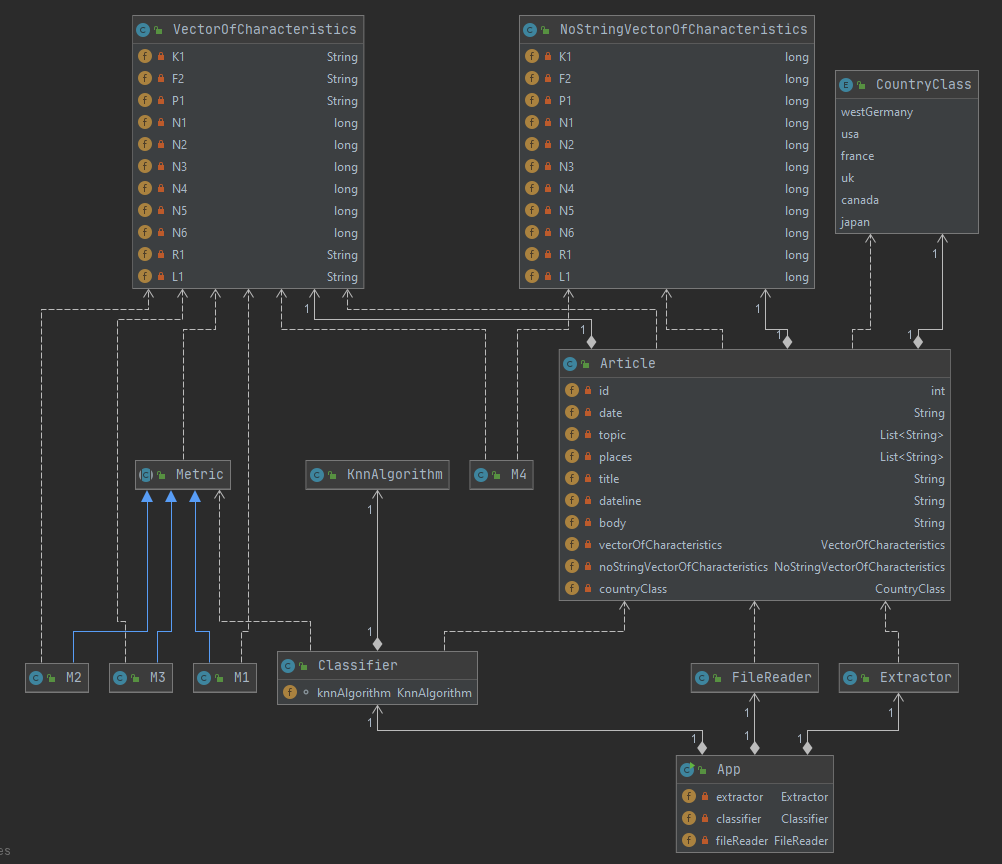
\includegraphics[width=0.66\textwidth]{uml1.png}
\caption{Diagram UML klas aplikacji, wraz z ich parametrami}
\label{fig1}
\end{figure}

Ideą aplikacji jest jej prostota (sposóbu użycia, wyglądu, zapisu danych) oraz rozłożenie logiki na 3 główne moduły (klasy): 
\begin{enumerate}
\item moduł FileReader - moduł odpowiadający za operacje na plikach i danych w nich zawartych. Pobiera dane z plików tekstowych, \cite{teksty} a następnie mapuje je na model klasy Article
\item moduł Extractor - moduł odpowiadający za ekstrakcje wektorów cech z każdego dokumentu tekstowego przedstawionego za pomocą klasy Article
\item moduł Classifier - moduł odpowiadający za klasyfikacje dokumentów (klasy Article) na podstawie ich wektorów cech za pomocą algorytmu KNN \cite{tadeusiewicz90} (klasa KnnAlgorithm) i jednej z wybranych przez użytkownika metryk (klasy M1, M2, M3)
\end{enumerate}

\subsection{Prezentacja wyników, interfejs użytkownika}  
%in - k, proporcje zbiorów na uczącuy i testowy, wybór miary i/lub metryki podobieństwa
%out - parametry, 
Aplikacja komunikuje sie z użytkownikiem za pomocą konsolowego interfejsu. Na początku działania programu użytkownik proszony jest o podanie parametrów takich jak:  
wartość $k$, określająca liczbę sąsiadów stosowanych w algorytmie klasyfikującym; 
procent zbioru dokumentów, który ma stanowić zbiór uczący, a także wybiera miary/metryki podobieństwa wektorów cech. Wybór parametrów wejściowych odbywa się poprzez podanie
cyfry/litery odpowiadającej jednemu z możliwych do wyboru wariantów, w przypadku wyboru miar/metryk. Natomiast jako wartość zmiennej $k$, jak i podział zbioru na uczący i testowy, jest podana przez użytkownika liczba całkowita mieszcząca się w podanym zakresie.
Po zakończeniu klasyfikacji wyniki wraz z obliczonymi miarami jakości klasyfikacji zostają wyświetlone w konsolowym interfejsie oraz zapisane do pliku tekstowego o wybranej przez użytkownika nazwie bądź domyślnie o nazwie: \textbf{"results.txt"}

Aplikacja jest uruchamiana z linii poleceń, wymagane jest posiadanie JDK w wersji 17. 

% Krótki ilustrowany opis jak użytkownik może korzystać z aplikacji, w~szczególności wprowadzać parametry klasyfikacji i odczytywać wyniki. Wersja JRE i inne wymogi
% niezbędne do uruchomienia aplikacji przez użytkownika na własnym komputerze. \\
% \noindent {\bf Sekcja uzupełniona jako efekt zadania Tydzień 04 wg Harmonogramu Zajęć
% na WIKAMP KSR.}

\section{Wyniki klasyfikacji dla różnych parametrów wejściowych}
%Wyniki kolejnych eksperymentów wg punktów 2.-8. opisu projektu 1.  Wykresy i tabele
%obowiązkowe, dokładnie opisane w ,,captions'' (tytułach), konieczny opis osi i
%jednostek wykresów oraz kolumn i wierszy tabel.\\ 

%{**Ewentualne wyniki realizacji punktu 9. opisu Projektu 1., czyli,,na ocenę 5.0'' i ich porównanie do wyników z
%części obowiązkowej**.}\\

%\noindent {\bf Sekcja uzupełniona jako efekt zadania Tydzień 05 wg Harmonogramu Zajęć
%na WIKAMP KSR.}

Poniżej zamieszczono tabele wynikowe oraz wykresy zależności miary Accuracy od poszczególnych parametrów:

\begin{table}[!htbp]
    \centering
\caption{Tabela zawierająca wyniki klasyfikacji w zależności od wartości parametru k algorytmu KNN dla metryki M2, 8000 dokumentów oraz dla klasyfikacji 30\% zbioru artykułów (70\% dokumentów należało do zbioru uczącego). Wykres zawiera linię trendu wykazającą wspomnianą zależność}
\begin{adjustbox}{max width=\textwidth}
    \begin{tabular}{|l|l|l|l|l|l|l|l|l|l|l|l|l|l|l|l|l|}
    \hline
        K & Acc & PPVc & TPRc & F1c & PPV & ~ & ~ & ~ & ~ & ~ & TPR & ~ & ~ & ~ & ~ & ~ \\ \hline
        ~ & ~ & ~ & ~ & ~ & west-germany  & usa  & japan & france & uk & canada & west-germany  & usa  & japan & france & uk & canada \\ \hline
        2 & 0.7597 & 0.5923 & 0.7549 & 0.6635 & 0.0000 & 0.7627 & 0.0061 & 0.0000 & 0.0038 & 0.0073 & 0.0000 & 0.9732 & 0.0012 & 0.0000 & 0.0012 & 0.0024 \\ \hline
        3 & 0.7606 & 0.5921 & 0.7573 & 0.6641 & 0.0000 & 0.7619 & 0.0205 & 0.0000 & 0.0036 & 0.0036 & 0.0000 & 0.9764 & 0.0035 & 0.0000 & 0.0012 & 0.0012 \\ \hline
        4 & 0.7712 & 0.6000 & 0.7684 & 0.6734 & 0.0000 & 0.7721 & 0.0208 & 0.0000 & 0.0037 & 0.0040 & 0.0000 & 0.9907 & 0.0036 & 0.0000 & 0.0012 & 0.0012 \\ \hline
        5 & 0.7720 & 0.5997 & 0.7705 & 0.6742 & 0.0000 & 0.7724 & 0.0069 & 0.0000 & 0.0000 & 0.0081 & 0.0000 & 0.9935 & 0.0012 & 0.0000 & 0.0000 & 0.0025 \\ \hline
        6 & 0.7751 & 0.6016 & 0.7744 & 0.6769 & 0.0000 & 0.7751 & 0.0070 & 0.0000 & 0.0039 & 0.0000 & 0.0000 & 0.9986 & 0.0012 & 0.0000 & 0.0012 & 0.0000 \\ \hline
        7 & 0.7753 & 0.6016 & 0.7749 & 0.6772 & 0.0000 & 0.7752 & 0.0070 & 0.0000 & 0.0039 & 0.0000 & 0.0000 & 0.9993 & 0.0012 & 0.0000 & 0.0012 & 0.0000 \\ \hline
        8 & 0.7753 & 0.6011 & 0.7753 & 0.6772 & 0.0000 & 0.7753 & 0.0000 & 0.0000 & 0.0000 & 0.0000 & 0.0000 & 1.0000 & 0.0000 & 0.0000 & 0.0000 & 0.0000 \\ \hline
        9 & 0.7753 & 0.6011 & 0.7753 & 0.6772 & 0.0000 & 0.7753 & 0.0000 & 0.0000 & 0.0000 & 0.0000 & 0.0000 & 1.0000 & 0.0000 & 0.0000 & 0.0000 & 0.0000 \\ \hline
        10 & 0.7753 & 0.6011 & 0.7753 & 0.6772 & 0.0000 & 0.7753 & 0.0000 & 0.0000 & 0.0000 & 0.0000 & 0.0000 & 1.0000 & 0.0000 & 0.0000 & 0.0000 & 0.0000 \\ \hline
        11 & 0.7753 & 0.6011 & 0.7753 & 0.6772 & 0.0000 & 0.7753 & 0.0000 & 0.0000 & 0.0000 & 0.0000 & 0.0000 & 1.0000 & 0.0000 & 0.0000 & 0.0000 & 0.0000 \\ \hline
    \end{tabular}
\end{adjustbox}
\end{table}

\begin{table}[!htbp]
    \centering
\caption{Tabela zawierająca wyniki klasyfikacji w zależności od wartości procentowej zbioru klasyfikowanego dla metryki M1, 8000 dokumentów oraz dla wartości parametru k algorytmu KNN równej 5. Wykres zawiera linię trendu wykazającą wspomnianą zależnośćć}
\begin{adjustbox}{max width=\textwidth}
    \begin{tabular}{|l|l|l|l|l|l|l|l|l|l|l|l|l|l|l|l|l|}
    \hline
        Split (\%) & Acc & PPVc & TPRc & F1c & PPV & ~ & ~ & ~ & ~ & ~ & TPR & ~ & ~ & ~ & ~ & ~ \\ \hline
        ~ & ~ & ~ & ~ & ~ & west-germany  & usa  & japan & france & uk & canada & west-germany  & usa  & japan & france & uk & canada \\ \hline
        10 & 0.7910 & 0.6341 & 0.7889 & 0.7027 & 0.0000 & 0.7913 & 0.0000 & 0.0000 & 0.0227 & 0.0033 & 0.0000 & 0.9865 & 0.0000 & 0.0000 & 0.0073 & 0.0011 \\ \hline
        20 & 0.7921 & 0.6332 & 0.7907 & 0.7032 & 0.0000 & 0.7930 & 0.0000 & 0.0000 & 0.0037 & 0.0000 & 0.0000 & 0.9906 & 0.0000 & 0.0000 & 0.0012 & 0.0000 \\ \hline
        30 & 0.7927 & 0.6338 & 0.7915 & 0.7037 & 0.0000 & 0.7933 & 0.0084 & 0.0000 & 0.0042 & 0.0000 & 0.0000 & 0.9913 & 0.0013 & 0.0000 & 0.0014 & 0.0000 \\ \hline
        40 & 0.7864 & 0.6227 & 0.7850 & 0.6941 & 0.0000 & 0.7864 & 0.0206 & 0.0000 & 0.0000 & 0.0102 & 0.0000 & 0.9930 & 0.0030 & 0.0000 & 0.0000 & 0.0031 \\ \hline
        50 & 0.7841 & 0.6203 & 0.7812 & 0.6913 & 0.0000 & 0.7858 & 0.0111 & 0.0000 & 0.0056 & 0.0000 & 0.0000 & 0.9907 & 0.0018 & 0.0000 & 0.0018 & 0.0000 \\ \hline
    \end{tabular}
\end{adjustbox}
\end{table}

\begin{table}[!htbp]
    \centering
\caption{Tabela zawierająca wyniki klasyfikacji w zależności od wybranej metryki dla 8000 dokumentów, wartości parametru k algorytmu KNN równej 5 oraz dla klasyfikacji 30\% zbioru artykułów (70\% dokumentów należało do zbioru uczącego).}
\begin{adjustbox}{max width=\textwidth}
    \begin{tabular}{|l|l|l|l|l|l|l|l|l|l|l|l|l|l|l|l|l|}
    \hline
        Metryka & Acc & PPVc & TPRc & F1c & PPV & ~ & ~ & ~ & ~ & ~ & TPR & ~ & ~ & ~ & ~ & ~ \\ \hline
        ~ & ~ & ~ & ~ & ~ & west-germany  & usa  & japan & france & uk & canada & west-germany  & usa  & japan & france & uk & canada \\ \hline
        M1 & 0.7836 & 0.6181 & 0.7818 & 0.6901 & 0.0000 & 0.7843 & 0.0000 & 0.0000 & 0.0112 & 0.0042 & 0.0000 & 0.9933 & 0.0000 & 0.0000 & 0.0039 & 0.0013 \\ \hline
        M2 & 0.7836 & 0.6181 & 0.7818 & 0.6901 & 0.0000 & 0.7843 & 0.0000 & 0.0000 & 0.0112 & 0.0042 & 0.0000 & 0.9933 & 0.0000 & 0.0000 & 0.0039 & 0.0013 \\ \hline
        M3 & 0.7836 & 0.6181 & 0.7818 & 0.6901 & 0.0000 & 0.7843 & 0.0000 & 0.0000 & 0.0112 & 0.0042 & 0.0000 & 0.9933 & 0.0000 & 0.0000 & 0.0039 & 0.0013 \\ \hline
    \end{tabular}
\end{adjustbox}
\end{table}

\begin{table}[!htbp]
    \centering
\caption{Tabela zawierająca wyniki klasyfikacji w zależności od wybranych podzbiorów cech używanych w obliczeniach odległości w algorytmie KNN dla 8000 dokumentów, klasyfikacji 30\% zbioru artykułów (70\% dokumentów należało do zbioru uczącego), wartości parametru k algorytmu KNN równej 5 oraz dla metryki M1.}
\begin{adjustbox}{max width=\textwidth}
    \begin{tabular}{|l|l|l|l|l|l|l|l|l|l|l|l|l|l|l|l|l|}
    \hline
        Podzbiór cech & Acc & PPVc & TPRc & F1c & PPV & ~ & ~ & ~ & ~ & ~ & TPR & ~ & ~ & ~ & ~ & ~ \\ \hline
        ~ & ~ & ~ & ~ & ~ & west-germany  & usa  & japan & france & uk & canada & west-germany  & usa  & japan & france & uk & canada \\ \hline
        N1, N2, N3, N4, N5, N6 & 0.7927 & 0.6283 & 0.7927 & 0.7010 & 0.0000 & 0.7927 & 0.0000 & 0.0000 & 0.0000 & 0.0000 & 0.0000 & 1.0000 & 0.0000 & 0.0000 & 0.0000 & 0.0000 \\ \hline
        K1, F2, P1, R1, L1 & 0.7962 & 0.6371 & 0.7954 & 0.7074 & 0.0000 & 0.7965 & 0.0082 & 0.0000 & 0.0000 & 0.0000 & 0.0000 & 0.9948 & 0.0014 & 0.0000 & 0.0000 & 0.0000 \\ \hline
        R1, L1 & 0.8003 & 0.6461 & 0.7998 & 0.7147 & 0.0000 & 0.8005 & 0.0079 & 0.0000 & 0.0000 & 0.0000 & 0.0000 & 0.9914 & 0.0014 & 0.0000 & 0.0000 & 0.0000 \\ \hline
        K1, F2, P1, N1, N2, N3, N4, N5, N6 & 0.7847 & 0.6158 & 0.7847 & 0.6901 & 0.0000 & 0.7847 & 0.0000 & 0.0000 & 0.0000 & 0.0000 & 0.0000 & 1.0000 & 0.0000 & 0.0000 & 0.0000 & 0.0000 \\ \hline
    \end{tabular}
\end{adjustbox}
\end{table}

\begin{figure}[!htbp]
\centering
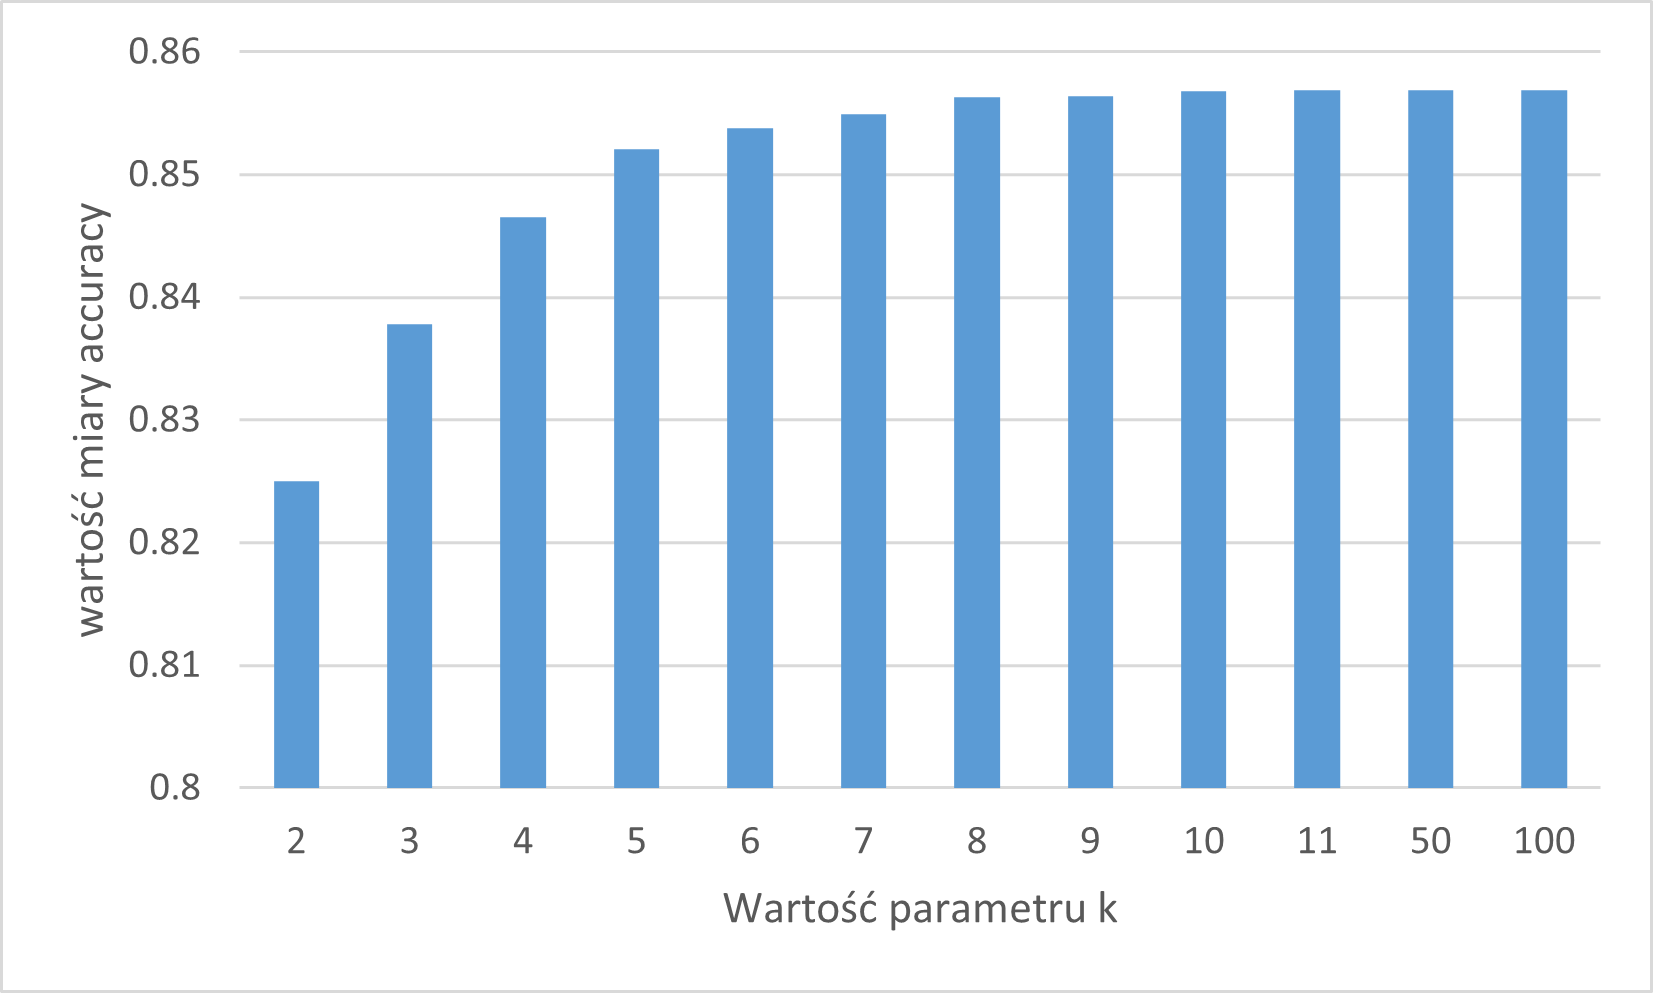
\includegraphics[width=0.66\textwidth]{wykres5.png}
\caption{Wykres zależności miary Accuracy od wartości parametru k algorytmu KNN dla metryki M2, 8000 dokumentów oraz dla klasyfikacji 30\% zbioru artykułów (70\% dokumentów należało do zbioru uczącego). Wykres zawiera linię trendu wykazającą wspomnianą zależność.}
\end{figure}

\begin{figure}[!htbp]
\centering
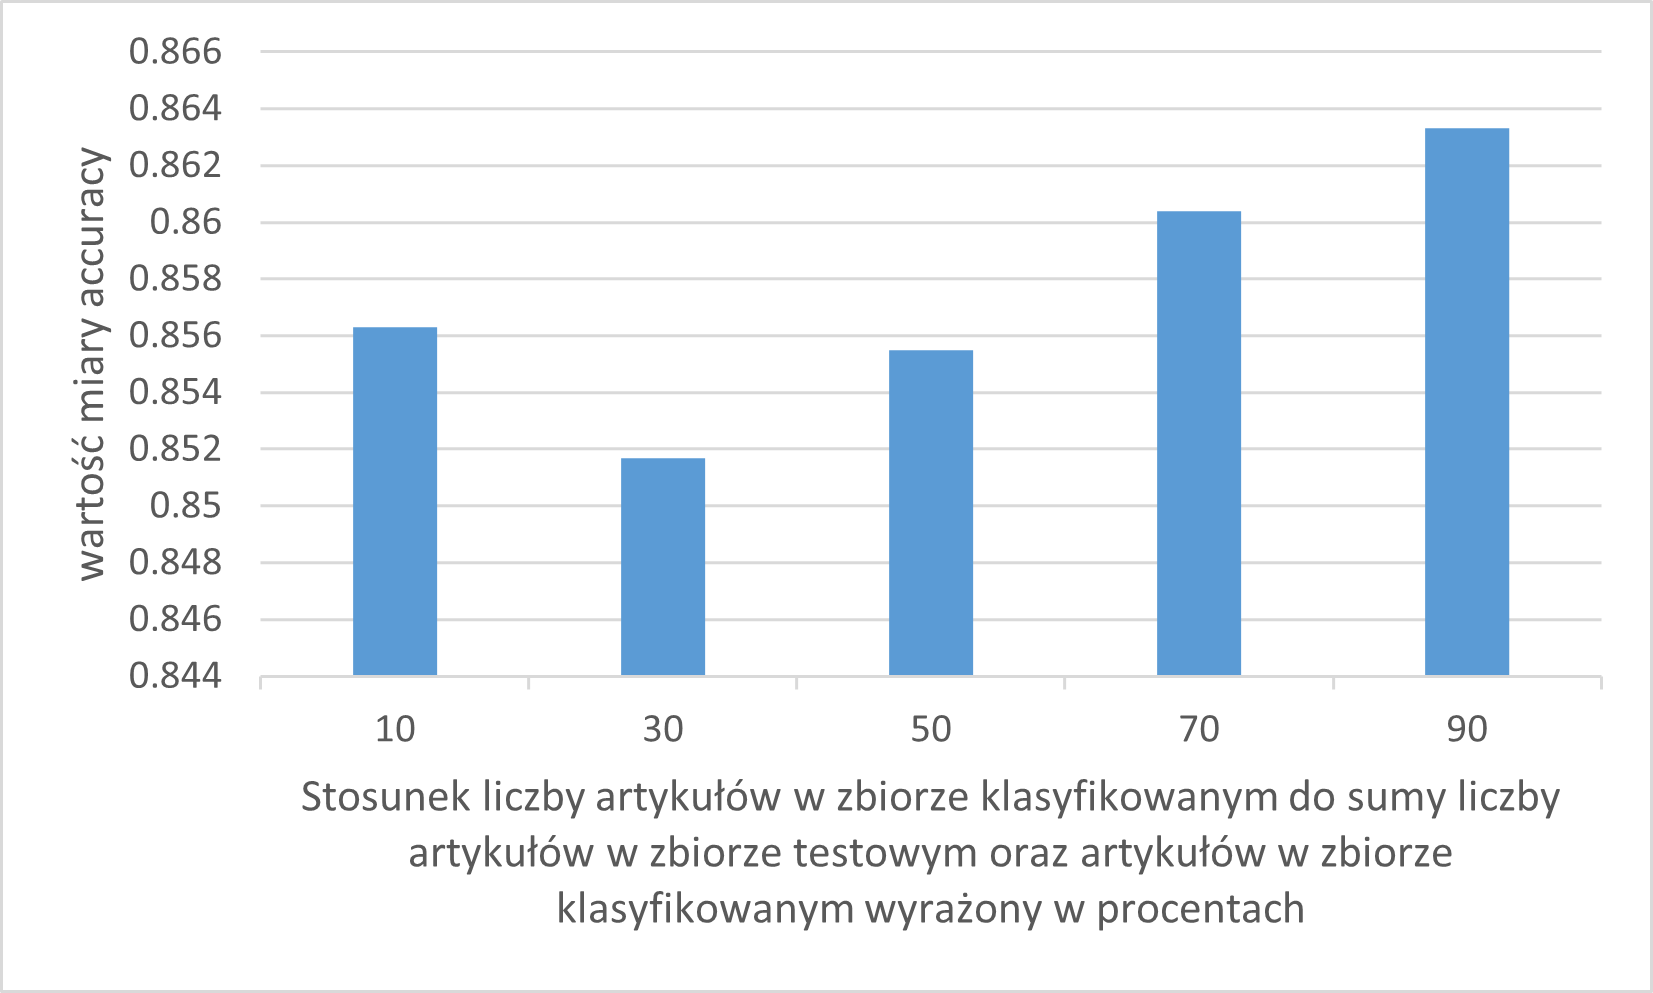
\includegraphics[width=0.66\textwidth]{wykres6.png}
\caption{Wykres zależności miary Accuracy od wartości procentowej zbioru klasyfikowanego dla metryki M1, 8000 dokumentów oraz dla wartości parametru k algorytmu KNN równej 5. Wykres zawiera linię trendu wykazającą wspomnianą zależność}
\end{figure}

\begin{figure}[!htbp]
\centering
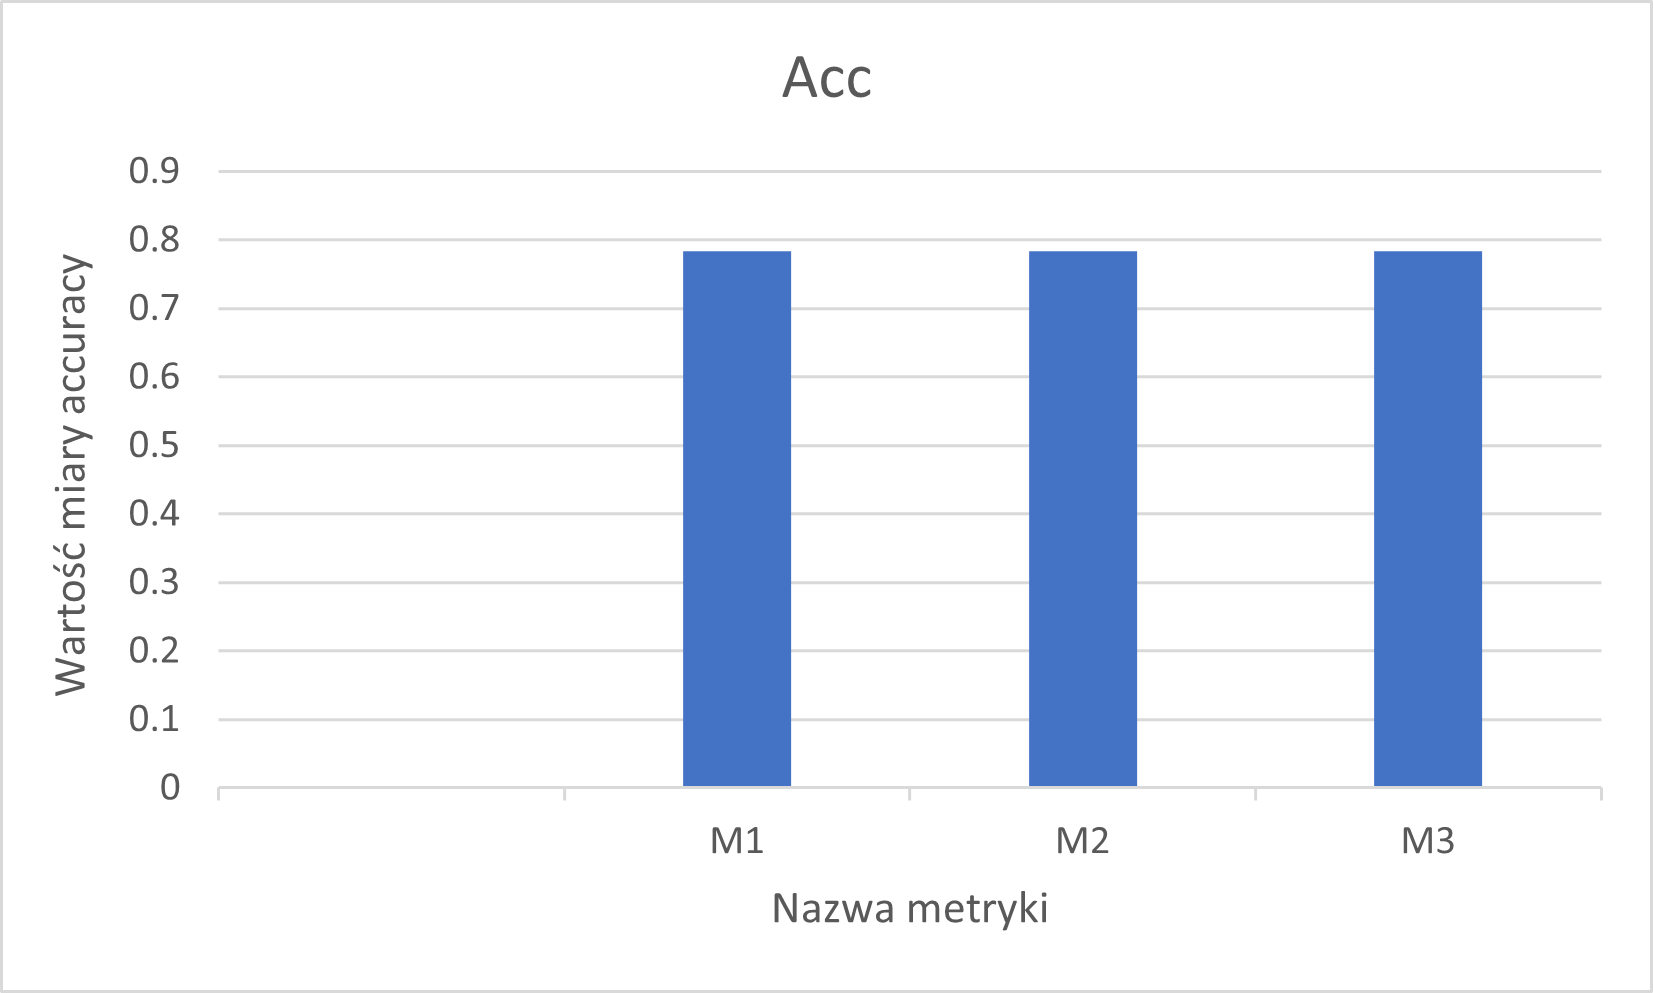
\includegraphics[width=0.66\textwidth]{wykres7.png}
\caption{Wykres zależności miary Accuracy od wybranej metryki dla 8000 dokumentów, wartości parametru k algorytmu KNN równej 5 oraz dla klasyfikacji 30\% zbioru artykułów (70\% dokumentów należało do zbioru uczącego).}
\end{figure}

\begin{figure}[!htbp]
\centering
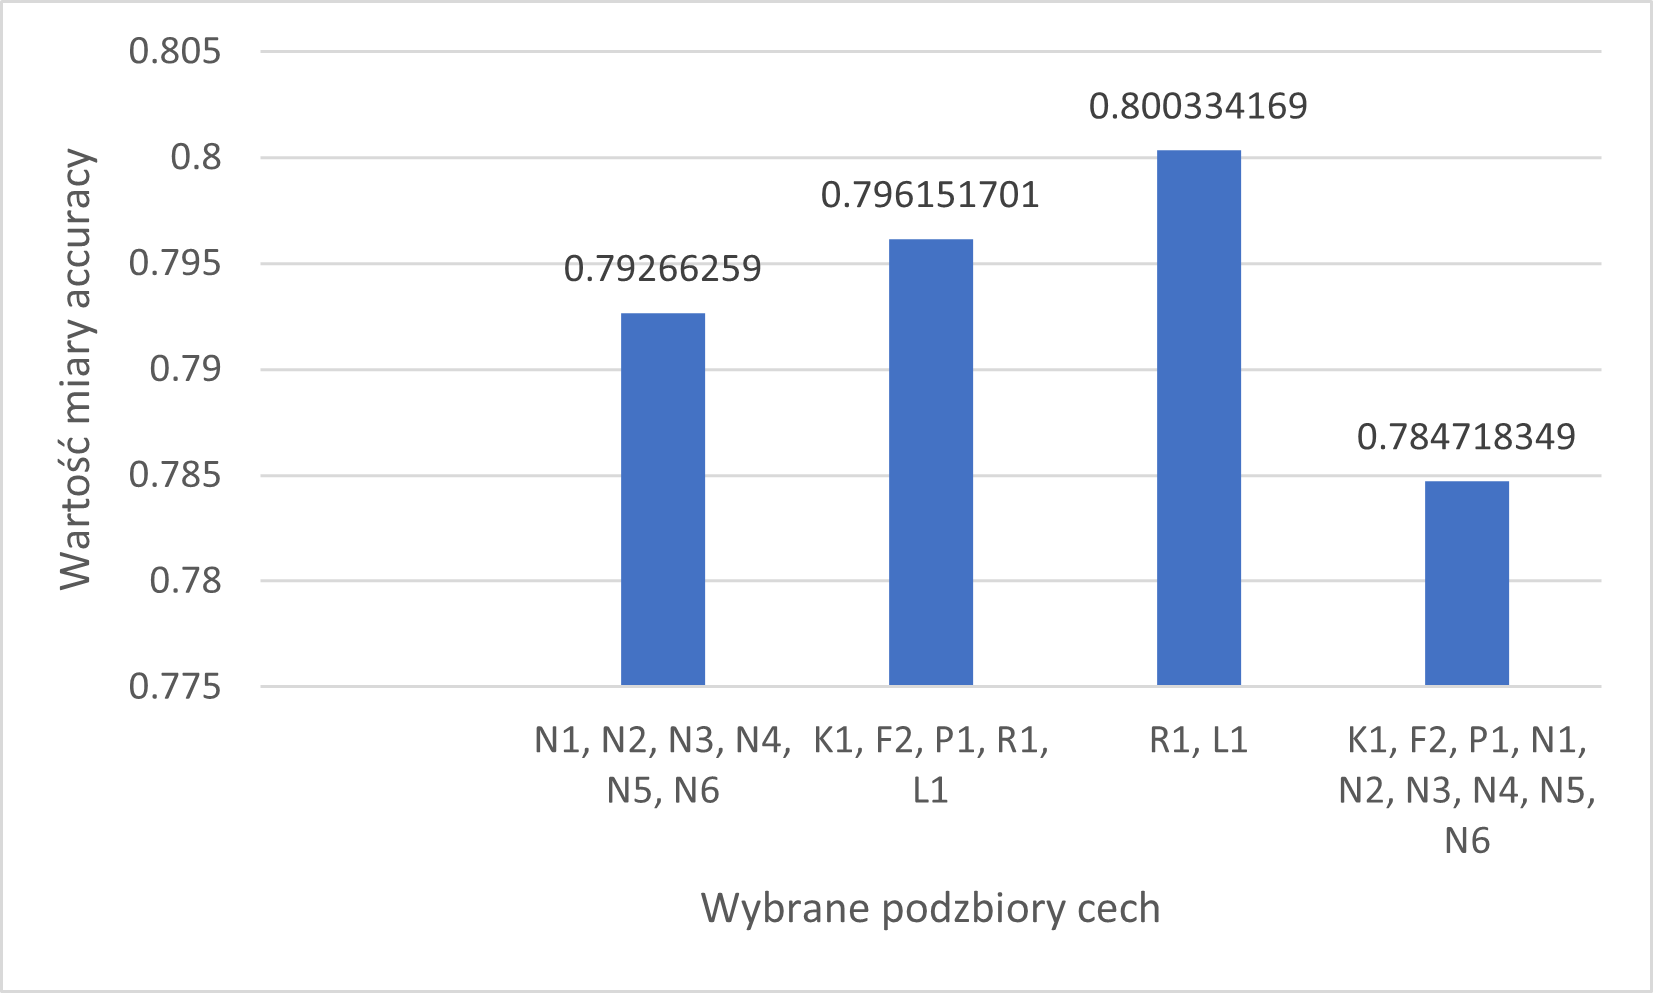
\includegraphics[width=0.66\textwidth]{wykres8.png}
\caption{Wykres zależności miary Accuracy od wybranych podzbiorów cech używanych w obliczeniach odległości w algorytmie KNN dla 8000 dokumentów, klasyfikacji 30\% zbioru artykułów (70\% dokumentów należało do zbioru uczącego), wartości parametru k algorytmu KNN równej 5 oraz dla metryki M1.}
\end{figure}


\section{Dyskusja, wnioski}
Dokładne interpretacje uzyskanych wyników w zależności od parametrów klasyfikacji
opisanych w punktach 3.-8 opisu Projektu 1. 
Szczególnie istotne są wnioski o charakterze uniwersalnym, istotne dla podobnych zadań. 
Omówić i wyjaśnić napotkane problemy (jeśli były). Każdy wniosek/problem powinien mieć poparcie
w przeprowadzonych eksperymentach (odwołania do konkretnych wyników: wykresów,
tabel). \\
\underline{Dla końcowej oceny jest to najważniejsza sekcja} sprawozdania, gdyż prezentuje poziom
zrozumienia rozwiązywanego problemu.\\

** Możliwości kontynuacji prac w obszarze systemów rozpoznawania, zwłaszcza w kontekście pracy inżynierskiej,
magisterskiej, naukowej, itp. **\\

\noindent {\bf Sekcja uzupełniona jako efekt zadania Tydzień 06 wg Harmonogramu Zajęć
na WIKAMP KSR.}


\section{Braki w realizacji projektu 1.}
Wymienić wg opisu Projektu 1. wszystkie niezrealizowane obowiązkowe elementy projektu, ewentualnie
podać merytoryczne (ale nie czasowe) przyczyny tych braków. 


\begin{thebibliography}{0}
\bibitem{tadeusiewicz90} R. Tadeusiewicz: Rozpoznawanie obrazów, PWN, Warszawa, 1991.  
\bibitem{niewiadomski08} A. Niewiadomski, Methods for the Linguistic Summarization of Data: Applications of Fuzzy Sets and Their Extensions, Akademicka Oficyna Wydawnicza EXIT, Warszawa, 2008.
\bibitem{teksty} http://archive.ics.uci.edu/ml/datasets/Reuters-21578+Text+Categorization+Collection
\bibitem{tablicapomylek} https://pl.wikipedia.org/wiki/Tablica\textunderscore pomyłek
\bibitem{slowniki} dictonaries.txt - plik załączany wraz z raportem, zawierający słowniki użyte w projekcie.
\end{thebibliography}

Literatura zawiera wyłącznie źródła recenzowane i/lub o potwierdzonej wiarygodności,
możliwe do weryfikacji i cytowane w sprawozdaniu. 
\end{document}